\svnidlong
{$HeadURL$}
{$LastChangedDate$}
{$LastChangedRevision$}
{$LastChangedBy$}
\svnid{$Id: $}

\chapter{Experimental}
\label{ch:Experimental}


\section{Colloid synthesis}
\label{sec:synthesis}

Our method to synthesize fluorescently labeled and sterically stabilized \ac{PMMA} colloids is mainly based on the Pine sythesis~\citep{klein2003} but is also inspired of works by \citet{antl1986} and \citet{bosma2002}.


\subsection{Principle}

The principle of this colloid synthesis is a well controlled polymerization of Methyl-Methacrylate. The monomer dissolves easily into an apolar solvent such as Hexane. But at a certain degree of polymerization, the polymer chain becomes immiscible and collapses on itself, forming a nucleus for the colloid growth. Until the monomer is completely consumed in the reactor, the nuclei continue to grow. The growth rate is determined by the concentration of monomer and is therefore uniform for a well-stirred reactor. So, all colloid nucleus should appear at the same time, grow at the same rate and stop their growth at the same moment. This allows a production of fairly monodisperse colloids.

But the nuclei being immiscible in the solvent, they would tend to aggregate, forming a block of \ac{PMMA} instead of well dispersed spheres. Which is why the colloids must be stabilized. The stabilizer is a large molecule with a functional group looking like the monomer in order to get involved in the polymerization. That way the stabilizer is chemically bonded to the colloid and pointing outward, sterically repelling the other colloids. Therefore colloids are no longer able to aggregate, as explained in \SectionRef{sec:HS-colloids}. We used methacryloxypropyl terminated \ac{PDMS} (Mw = \unit{25000}{\gram\per\mole}) as stabilizer.

In order to get fluorescently labeled colloids, some synthesis methods only add the fluorescent dye into the reaction mixture. The dye is then trapped physically into the growing colloids, and once washed, the colloids are fluorescently labeled. The problem with this method is that the labeling is unstable. After some time in a solvent, the dye diffuses out of the colloids, leading to a more and more fluorescent solvent, to less and less fluorescent colloids and so to worse and worse quality of imaging of the sample. To avoid that, we functionalized our dyes (rhodamine B isothiocyanate or coumarine) with a methacrylate group able to polymerize into \ac{PMMA} chains. That way, we get a dye chemically bonded to the colloids and a very stable labeling.


\subsection{Experimental procedure}


\subsubsection{Preparation of the ingredients}

In order to have a well controlled initiation of the polymerization reaction, a very pure initiator is needed. We used commercial \ac{ADIB} but we recrystallized it in acetone.

Commercial monomer \ac{MMA} is sold inhibited, in order to prevent any polymerization before use. The inhibitor must be removed before use, using an inhibitor remover column. The inhibited monomer is poured thought the column and comes out free of inhibitor.

The making of dyed monomer is also a part of the preparation. We mix \ac{EGDM} with the dye (rhodamine B isothiocyanate or coumarine) in acetone and stir it during two days in a UV-screened flask. The acetone is then evaporated to get back the dyed monomer as a powder.


\subsubsection{Experimental setup of the synthesis}

The synthesis was performed in a \unit{250}{\milli\litre} three-neck flask placed in a heated silicon oil bath and stirred magnetically. The flask was equipped with two removable caps to add chemicals and a water cooled reflux condenser topped by a nitrogen inlet tube to prevent oxygen diffusing into the system.

A typical synthesis proceeds as follow: Initially \unit{0.2}{\gram} of initiator was dissolved into \unit{44}{\gram} of hexane and \unit{22}{\gram} of dodecane (less volatile). Then \unit{0.2}{\gram} of stabilizer at \unit{25000}{\gram\per\mole} was added as well as a part of the monomer (in order to have around \unit{5}{\gram} of monomer remaining). Then the flask was set under the reflux and stirred. Meanwhile, the dye was dissolved into a mixture of \unit{0.8}{\gram} of acetone (to get higher polarity and higher solubility), \unit{0.41}{\gram} of \ac{MA} and the rest of the monomer. If the dye was overdosed, the non-dissolved bits where filtered off before the dyed mixture was poured into the reactor.

Finally, polymerization stopper (\unit{1}{\milli\litre} of octanethiol) was added into the reactor. After one minute of moderate nitrogen flux, all caps were sealed and the nitrogen flux stopped. The reaction mixture is then heated to \unit{80}{\celsius} for an hour. Before reaching this temperature, flocculation of densely dyed material may occur. In this case, the heating is stopped, the reaction mixture filtered and all is put back in the same configuration and heated again to \unit{80}{\celsius}. This filtering process was annoying but seemingly had no influence on the result of the synthesis.

After 1 hour at \unit{80}{\celsius} we let the reaction mixture cool down, sedimented into an Erlenmeyer flask and then washed two times with petroleum ether to keep only the colloids.


\subsection{Testing the synthesized colloids}


\subsubsection{Qualitatively by confocal microscope}

Just after reaction, a drop of the reaction mixture is dried on a microscope slide, immersed in a drop of index matched emulsion oil and then put under the confocal microscope. Dried colloids tend to form crystals. Measuring the lattice size of those crystals gives us a qualitative idea of the size of our particles.


\subsubsection{Quantitatively by light scattering}

Static light scattering spectrum of a drop of the reaction mixture diluted in hexane is fitted to Mie theory~\citep{Bohren1983, Dhont1996}. This gives us the mean size and the polydispersity of our colloids.


\subsection{Results of the synthesis}

The different parameters we used for the synthesis and the corresponding results are given in \TableRef{tab:Result-of-synthesis}. Only the two last syntheses and the two syntheses using coumarine dye did not need filtering. We were able to obtain diameters between \unit{0.98}{\micro\meter} and \unit{1.58}{\micro\meter} with polydispersity between $4\%$ and $6.5\%$. We tried to broaden the diameter range in the last synthesis by quenching the reaction after \unit{11}{\minute} at \unit{80}{\celsius}. We could then obtain a diameter of \unit{0.38}{\micro\meter} but with a $12\%$ polydispersity.


\begin{sidewaystable}
	\centering
	
	\begin{tabular}{|r|c|c|c|c|c|c|c|c|c|c|}
	\hline RAS & \milli\gram & $\sim$25 & $\sim$25 & $\sim$25 &  &  & 13 & 5.2 & 5.8 & 5.9 \\ 
	\hline CAS & \milli\gram &  &  &  & $\sim$25 & 10.7 &  &  &  &  \\ 
	\hline \ac{ADIB} & \gram & 0.2 & 0.2 & 0.2 & 0.2 & 0.205 & 0.204 & 0.102 & 0.2054 & 0.103 \\ 
	\hline Hexane & \gram & 44 & 44 & 44 & 44 & 44.04 & 44.02 & 44 & 44.01 & 44.02 \\ 
	\hline Dodecane & \gram & 22 & 22 & 22 & 22 & 22 & 22.08 & 22.01 & 22 & 22.25 \\ 
	\hline \ac{MMA} & \gram & 20.3 & 20.3 & 20.3 & 20.3 & 20.31 & 20.29 & 10.1 & 10.04 & 10.08 \\ 
	\hline \ac{MA} & \gram & 0.4 & 0.4 & 0.4 & 0.4 & 0.41 & 0.41 & 0.22 & 0.1985 & 0.2 \\ 
	\hline acetone & \gram & 0.8 & 0.8 & 0.87 & 0.8 & 0.8 & 0.8 & 0.44 & 0.8 & 0.42 \\ 
	\hline stabilizer & \gram & 1 & 0.58 & 0.38 & 1.18 & 0.69 & 1.7 & 0.52 & 1.71 & 0.99 \\ 
	\hline octanthiol & \milli\litre & 0.1 & 0.1 & 0.1 & 0.1 & 0.1 & 0.1 & 0.05 & 0.1 & 0.1 \\ 
	\hline $\sigma$ & \micro\metre & 1.22 & 1.46 & 1.58 & 1.10 & 1.52 & 1.03 & 1.15 & 0.98 & 0.38 \\ 
	\hline $\Delta$ & $\%$ & 6 & 5 & 5 & 6 & 6.5 & 6.5 & 4 & 4 & 12 \\ 
	\hline 
	\end{tabular} 
	
	\caption{Result of colloid synthesis. The last one was quenched after 11 min. RAS stands for methacrylated rhodamine, CAS for methacrylated coumarine.}
	\label{tab:Result-of-synthesis}
\end{sidewaystable}

\section{Experimental setup}


\subsection{Samples}
\label{sec:samples}

\subsubsection{Hard Spheres colloids}
\label{subsec:colloids}
We used \ac{PMMA} colloids synthesised following the protocol detailed in \SectionRef{sec:synthesis}. The colloids are sterically stabilized with methacryloxypropyl terminated PDMS and fluorescently labelled with rhodamine isothiocyanate chemically bonded to the \ac{PMMA}~\citep{bosma2002}.

The colloids are suspended in a solvent mixture of \ac{CIS} and \ac{CHB}. Both solvents have a refractive index close to the one of \ac{PMMA} ($n_{PMMA}=1.4947$, $n_{CIS}=1.481$, $n_{CHB}=1.5052$). Refractive index matching enables us to see through a few millimetres of concentrated suspensions without suffering from multiple scattering of light and leads to very precise imaging hundreds of microns deep into our samples. Due to the steric stabilization and refractive index matching, the van der Waals interactions are reduced to a fraction of the thermal energy and can therefore be neglected. 

To screen any (weak) electrostatic interactions, we dissolved \ac{TBAB} salt, to a concentration of \unit{300}{\nano\mole\per\liter}~\citep{royall2005}. The estimated Debye screening length is \unit{100}{\nano\metre}, well below the length scale of the colloids. 

To the extent of our knowledge, the interactions between the colloids we used are as close as possible to the theoretical hard core potential for micron-sized particles.


\subsection{Size and polydispersity}
\label{sec:size_poly}
\subsubsection{On the importance of size}

Particle size determination is crucial for experiments. We saw in \SectionRef{sec:colloidalHS} that the phase behaviour and the glass transition of hard spheres is controlled by the volume fraction $\phi$ that is the volume of space occupied by the particles.
\begin{equation}
	\phi \equiv \sum_i \frac{\pi}{6}\frac{\sigma_i^3}{V} = \frac{\pi}{6}\langle \sigma^3 \rangle \rho
	\label{eq:volume-fraction}
\end{equation}
with $V$ the total volume, $\sigma_i$ the diameter of the particle $i$, and $\rho=N/V$ the number density. Our only way to know the volume fraction in the part of the sample we are observing is to measure $\rho$ by particle tracking and deduce $\phi$ using \EquationRef{eq:volume-fraction}. Thus an uncertainty of $1\%$ in the particle size results in a $3\%$ uncertainty in the volume fraction. Moreover, if in the case of monodisperse particles we have $\langle \sigma^3 \rangle = \langle \sigma \rangle^3$, this is not true in the general case. We define an effective diameter $\sigma_{eff} \equiv \sqrt[3]{\langle \sigma^3 \rangle}$.

\subsubsection{Sizing dry particles}
Dry particles were imaged with a \acf{SEM} (see \FigureRef{fig:SEM}). From these images we performed a sizing analysis of about 200 particles yielding an average dry radius of $\sigma=\unit{3.011}{\micro\meter}$ and a polydispersity of $\Delta=6.15\%$. The effective diameter is estimated to $\sigma_{eff}=\unit{3.022}{\micro\meter}$. Because of secondary nucleation, quite a few small particles are present (skew is $\gamma=-1.7$, kurtosis is $\kappa=6.6$), shifting $\sigma_{eff}$ of about $1\%$ compared to the peak of the size distribution ($\sigma_{peak}\sim\unit{3.057}{\micro\meter}$).

The degree of polydispersity of our particles is in any case sufficient to prevent or to delay crystallization long enough to observe a stable supercooled phase (see \SectionRef{sec:size_poly}). In practice, we observed these colloids crystallizing only with the help of wall-induced layering.

\begin{figure}
	\centering
	\subfloat[A typical \ac{SEM} image]{\label{fig:SEMimage}\includegraphics[width=0.45\textwidth]{SEM}}
	\subfloat[Size distribution]{\label{fig:SEMdistrib}\resizebox{0.50\textwidth}{!}{\input{diameter_histogram}}}
	%\subfloat[Size distribution]{\label{fig:SEMdistrib}\rotatebox{-90}{\includegraphics[height=0.35\textwidth]{diameter_histogram}}}
	\caption{\acs{SEM} sizing of the dried colloids used in this thesis. The size distribution is extracted from 200 particles out of many \acs{SEM} images. Due to secondary nucleation, the distribution is stretched towards small sizes.}
	\label{fig:SEM}
\end{figure}

Unfortunately, \ac{PMMA} particles swell in the solvents we use~\citep{bosma2002, ohtsuka2008local}. The volume of a particle in the solvent should be about $30\%$ larger than the same dry particle. Moreover, the swelling can take several weeks, so the particle size changes over time. Therefore we used only particles that had spent a sufficiently long time in the same solvent mixtures as used in the experiments and we had to measure their effective radius \latin{in situ}. The shape of the volume distribution of the particles is not expected to change.

\subsubsection{\latin{In situ} hard core diameter}
The most straightforward method to measure the hard core diameter of spheres is to push them together and to measure the distance between their centres. Because we have the coordinate of each particle, we can calculate the most frequent inter-particular distance as the position of the first peak of the radial distribution function $g(r)$. If the colloids are at contact, the position of the first peak of $g(r)$ should give the most frequent diameter, \latin{i.e.} the mode of the size distribution. Then, given the size distribution measured by \ac{SEM}, we can recover the effective diameter in the solvent.

Because Brownian hard spheres are rarely at contact, even at high concentration, we added non-adsorbing polymers (polystyrene) to the suspension. Polymers induces depletion attraction~\citep{asakura1954}, thus driving many particles into contact and leading to an accurate position for the first peak of $g(r)$ (see \FigureRef{fig:rdf-contact}). The typical accuracy of particle tracking is \unit{0.1}{pixels}, \latin{e.g.} $\sim\sigma/100$ when one samples around \unit{10}{pixels} per diameters. Relative uncertainty on the volume fraction would be $3\%$ with this technique.

Here we find $\sigma_{peak}=\unit{3.295\pm0.03}{\micro\meter}$, thus $\sigma_{eff}=\unit{3.256\pm0.03}{\micro\meter}$.

\begin{figure}
	\resizebox{0.9\textwidth}{!}{% GNUPLOT: LaTeX picture with Postscript
\begingroup
  \makeatletter
  \providecommand\color[2][]{%
    \GenericError{(gnuplot) \space\space\space\@spaces}{%
      Package color not loaded in conjunction with
      terminal option `colourtext'%
    }{See the gnuplot documentation for explanation.%
    }{Either use 'blacktext' in gnuplot or load the package
      color.sty in LaTeX.}%
    \renewcommand\color[2][]{}%
  }%
  \providecommand\includegraphics[2][]{%
    \GenericError{(gnuplot) \space\space\space\@spaces}{%
      Package graphicx or graphics not loaded%
    }{See the gnuplot documentation for explanation.%
    }{The gnuplot epslatex terminal needs graphicx.sty or graphics.sty.}%
    \renewcommand\includegraphics[2][]{}%
  }%
  \providecommand\rotatebox[2]{#2}%
  \@ifundefined{ifGPcolor}{%
    \newif\ifGPcolor
    \GPcolortrue
  }{}%
  \@ifundefined{ifGPblacktext}{%
    \newif\ifGPblacktext
    \GPblacktexttrue
  }{}%
  % define a \g@addto@macro without @ in the name:
  \let\gplgaddtomacro\g@addto@macro
  % define empty templates for all commands taking text:
  \gdef\gplbacktext{}%
  \gdef\gplfronttext{}%
  \makeatother
  \ifGPblacktext
    % no textcolor at all
    \def\colorrgb#1{}%
    \def\colorgray#1{}%
  \else
    % gray or color?
    \ifGPcolor
      \def\colorrgb#1{\color[rgb]{#1}}%
      \def\colorgray#1{\color[gray]{#1}}%
      \expandafter\def\csname LTw\endcsname{\color{white}}%
      \expandafter\def\csname LTb\endcsname{\color{black}}%
      \expandafter\def\csname LTa\endcsname{\color{black}}%
      \expandafter\def\csname LT0\endcsname{\color[rgb]{1,0,0}}%
      \expandafter\def\csname LT1\endcsname{\color[rgb]{0,1,0}}%
      \expandafter\def\csname LT2\endcsname{\color[rgb]{0,0,1}}%
      \expandafter\def\csname LT3\endcsname{\color[rgb]{1,0,1}}%
      \expandafter\def\csname LT4\endcsname{\color[rgb]{0,1,1}}%
      \expandafter\def\csname LT5\endcsname{\color[rgb]{1,1,0}}%
      \expandafter\def\csname LT6\endcsname{\color[rgb]{0,0,0}}%
      \expandafter\def\csname LT7\endcsname{\color[rgb]{1,0.3,0}}%
      \expandafter\def\csname LT8\endcsname{\color[rgb]{0.5,0.5,0.5}}%
    \else
      % gray
      \def\colorrgb#1{\color{black}}%
      \def\colorgray#1{\color[gray]{#1}}%
      \expandafter\def\csname LTw\endcsname{\color{white}}%
      \expandafter\def\csname LTb\endcsname{\color{black}}%
      \expandafter\def\csname LTa\endcsname{\color{black}}%
      \expandafter\def\csname LT0\endcsname{\color{black}}%
      \expandafter\def\csname LT1\endcsname{\color{black}}%
      \expandafter\def\csname LT2\endcsname{\color{black}}%
      \expandafter\def\csname LT3\endcsname{\color{black}}%
      \expandafter\def\csname LT4\endcsname{\color{black}}%
      \expandafter\def\csname LT5\endcsname{\color{black}}%
      \expandafter\def\csname LT6\endcsname{\color{black}}%
      \expandafter\def\csname LT7\endcsname{\color{black}}%
      \expandafter\def\csname LT8\endcsname{\color{black}}%
    \fi
  \fi
  \setlength{\unitlength}{0.0500bp}%
  \begin{picture}(7200.00,5040.00)%
    \gplgaddtomacro\gplbacktext{%
      \csname LTb\endcsname%
      \put(1056,704){\makebox(0,0)[r]{\strut{}$0.0$}}%
      \put(1056,1383){\makebox(0,0)[r]{\strut{}$2.0$}}%
      \put(1056,2061){\makebox(0,0)[r]{\strut{}$4.0$}}%
      \put(1056,2740){\makebox(0,0)[r]{\strut{}$6.0$}}%
      \put(1056,3419){\makebox(0,0)[r]{\strut{}$8.0$}}%
      \put(1056,4097){\makebox(0,0)[r]{\strut{}$10.0$}}%
      \put(1056,4776){\makebox(0,0)[r]{\strut{}$12.0$}}%
      \put(1188,484){\makebox(0,0){\strut{}$0$}}%
      \put(1807,484){\makebox(0,0){\strut{}$1$}}%
      \put(2426,484){\makebox(0,0){\strut{}$2$}}%
      \put(3045,484){\makebox(0,0){\strut{}$3$}}%
      \put(3664,484){\makebox(0,0){\strut{}$4$}}%
      \put(4284,484){\makebox(0,0){\strut{}$5$}}%
      \put(4903,484){\makebox(0,0){\strut{}$6$}}%
      \put(5522,484){\makebox(0,0){\strut{}$7$}}%
      \put(6141,484){\makebox(0,0){\strut{}$8$}}%
      \put(6760,484){\makebox(0,0){\strut{}$9$}}%
      \put(286,2740){\rotatebox{90}{\makebox(0,0){\strut{}$g(r)$}}}%
      \put(6979,2740){\rotatebox{90}{\makebox(0,0){\strut{}}}}%
      \put(3974,154){\makebox(0,0){\strut{}$r (\micro\meter)$}}%
      \put(3974,4666){\makebox(0,0){\strut{}}}%
      \put(3974,4665){\makebox(0,0){\strut{}}}%
      \put(132,110){\makebox(0,0)[l]{\strut{}}}%
    }%
    \gplgaddtomacro\gplfronttext{%
      \csname LTb\endcsname%
      \put(5773,4548){\makebox(0,0)[r]{\strut{}Hard sphere supercooled liquid}}%
      \csname LTb\endcsname%
      \put(5773,4218){\makebox(0,0)[r]{\strut{}Colloid+polymer gel}}%
    }%
    \gplbacktext
    \put(0,0){\includegraphics{rdf_contact}}%
    \gplfronttext
  \end{picture}%
\endgroup
}
	\caption{Radial distribution function of a colloidal hard sphere supercooled liquid and of a dilute sample with added polymer (gel). In the gel, the position of the first peak is shifted to the shorter inter-particular distances, indicating that the particles are indeed at contact. First peaks positions are respectively \unit{3.473}{\micro\meter} and \unit{3.295}{\micro\meter}.}
	\label{fig:rdf-contact}
\end{figure}

%\subsubsection{\latin{In situ} hydrodynamic radius}


\subsection{Influence of gravity}

As introduced in \SectionRef{subsec:colloids} we use a mixture of two solvents. The main purpose of that is to control the colloid effective mass~\citep{royall2005}. \ac{PMMA} ($\rho_{PMMA}=\unit{1193}{\kilogrampercubicmetre}$) is heavier than cis-decalin ($\rho_{CIS}=\unit{897}{\kilogrampercubicmetre}$) but lighter than \ac{CHB} ($\rho_{CHB}=\unit{1335}{\kilogrampercubicmetre}$). Theoretically, the composition of the solvent mixture can be adjusted in order to perfectly match the density of the solvent with the density of the particles.

Two difficulties arise in practice: swelling of the particles and temperature dependence of the densities. \ac{PMMA} absorbs more \ac{CHB} than cis-decalin. This makes the particles lighter and the solvent heavier. So after some time in the solvent, the particles tend to settle down. We improved the density matching by centrifuging the solution, noting whether the particles settled upward or downward, and adding the appropriate solvent~\citep{dinsmore2001tdc}. Because the thermostat of our centrifuge was not precise enough($\pm \unit{1}{\celsius}$), the density match was yet not perfect. We then use the precise temperature controlled apparatus of the microscope (see \SectionRef{subsubsec:Tcontrol}) to find the temperature ($\pm \unit{0.1}{\celsius}$) achieving the best density match.


\subsection{Material}


\subsubsection{Principle of Confocal Microscopy\label{sub:Principle-of-Confocal}}

\begin{figure}
	\centering
	\def\svgwidth{\textwidth}\input{confocalprinciple_horizontal.pdf_tex}
	\caption{Principle of confocal microscopy. All light that do not come from the focal plane is stopped by the pinhole. Source Wikipedia.}
	\label{fig:Confocal_principle}
\end{figure}

The principle of confocal imaging was patented by Marvin Minsky in 1957~\citep{minsky1957}. Practical development of the idea awaited improvements in optics, electronics and data handling in the 60's, 70's and 80's. Confocal microscopy has now been used intensively in biology~\citep{Pawley2008} and in physics~ \citep{chestnut1997cmc} for about two decades. 

In a conventional (i.e., wide-field) fluorescence microscope, the entire specimen is flooded in light from a light source. Due to the conservation of light intensity transportation, all parts of the specimen throughout the optical path will be excited and the fluorescence detected by a photodetector or a camera. In contrast, a confocal microscope uses point illumination and a pinhole in an optically conjugate plane in front of the detector to eliminate out-of-focus information (see \FigureRef{fig:Confocal_principle}). Only the light within the focal plane can be detected, so the image quality is much better than that of wide-field images. As only one point is illuminated at a time in confocal microscopy, 2D or 3D imaging requires scanning over a regular raster (i.e. a rectangular pattern of parallel scanning lines) in the specimen. The thickness of the focal plane is defined mostly by the square of the numerical aperture of the objective lens, and also by the optical properties of the specimen and the ambient index of refraction.

In the following, we will refer to the scanning direction as $X$ and to the optical axis as $Z$ (corresponding to the direction of gravity, unless explicitly stated).


\subsubsection{Our material}
%
\begin{figure}
	\centering
	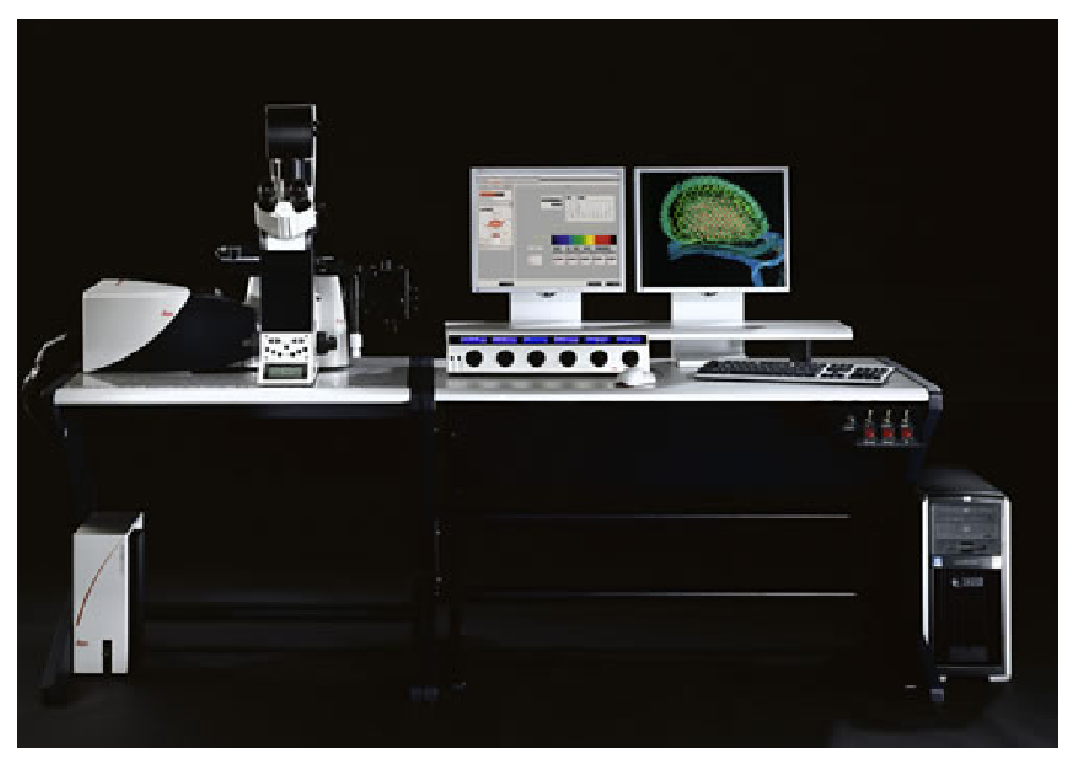
\includegraphics[width=0.5\textwidth]{Leica_SP5}
	\caption{Picture of a Leica SP5 confocal microscope without the temperature control apparatus.}
	\label{fig:Confocal}
\end{figure}


The data was collected on a Leica SP5 confocal microscope, using \unit{532}{\nano\meter} laser excitation. The sample was mounted on a galvano stage, allowing fast scanning in the $Z$ direction (sample is mobile, objective lens does not move). The typical pixel size is \unit{0.298}{\nano\meter} in all three dimensions, leading to a sampling of \unit{11}{pixels} per particle diameter for the most common particle sizes, and still about \unit{8}{pixels} for the smallest particles observed by SEM. The main advantage of using colloids as large as \unit{3}{\micro\meter} is that particles appear as well-defined disks on any 2D slice of the 3D image (see \FigureRef{fig:typical-slice}).

Leica SP5 fast scanner is able to scan with a frequency of \unit{8000}{\hertz}, meaning 8000 lines in a second. A stack of \unit{256}{pixels} in all three dimensions could be acquired in \unit{6}{\second}. On the other end of the spectrum, we were able to program the microscope to take a stack every 30 minutes during a few days. This allows us to follow the dynamics of our colloids through almost three orders of magnitude.

The colloidal suspension was filled into glass capillaries that were then sealed by UV glue. To prevent bleaching of the sample, the centre of the capillary was protected by aluminium foil while the ends were exposed to long wavelength ultra-violet light. We used both square section \unit{500}{\micro\metre} capillary cells and $\unit{100}{\micro\metre}\times\unit{1}{\milli\metre}$ capillary slits. Using an glycerol-immersed long working distance objective lens, we were able to image the whole depth of the slits, and to take data at least \unit{50}{\micro\meter} (\latin{i.e.} $>15\sigma$) far from any wall in the square capillaries.

\begin{figure}
	\centering
	\subfloat[$XY$ slice]{
\includegraphics[width=0.4\textwidth]{sliceXY}}\quad
	\subfloat[$XZ$ slice]{
\includegraphics[width=0.4\textwidth]{sliceXZ}}
	\caption{Detail of typical slices of a 3D image of a dense colloidal suspension.}
	\label{fig:typical-slice}
\end{figure}



\subsubsection{Temperature control}
\label{subsubsec:Tcontrol}

Because the sample was mounted on a galvano stage, thus moving precisely at a fast rate, the temperature control apparatus had to be lightweight, with the least inertia possible. On the other hand, we had no need of quick temperature variation. We decided to use only heaters and passive cooling by the air of the room. Then the sample had to be at higher temperature (around \unit{30}{\celsius}) than the room (around \unit{26}{\celsius}).

The sample was lying on a thermostated glass plate (ThermoPlate$\texttrademark$), custom-made by \emph{Tokai Hit Co., Ldt.} to be mounted on the Leica galvano stage. The objective lens was also thermostated because at contact with the sample through glycerol. Provided a temperature difference of at least \unit{2}{\celsius} between the room and the nominal temperature, the deviation from the nominal temperature was no more than \unit{0.1}{\celsius}.

%\newpage
% Create the bibliography right after the text
%\bibliographystyle{ieeetr}
%\bibliography{mathieu}